\chapter{Métodos y curvas de valoración}\label{ch:b1:titration-methods}

Una farmacéutica recibe un lote de comprimidos de vitamina C etiquetados
con \qty{500}{mg} y debe certificar, antes de venderlos, que cada uno
contiene lo que dice la etiqueta. No pesará la vitamina directamente: está
mezclada con aglutinantes y excipientes. La valorará: la hará reaccionar
con un reactivo de concentración conocida, medirá el volumen necesario y
calculará la cantidad. Qué reacción, cómo ver su final y qué seguridad
tiene el resultado: esas son las preguntas de este capítulo, que lleva a
la mesa del laboratorio los equilibrios de los cinco capítulos
anteriores.

\begin{recall}
El volumen escolar (años 11 y 12) valoró ácidos con bases mediante un
cambio de color, siguió \omterm{def:b1:titration-methods:titration}{valoraciones} con un pHmetro y con un
conductímetro, y usó la relación de \omterm{def:b1:titration-methods:titration}{equivalencia} $C_AV_A = C_BV_B$. El
método de la \omterm{def:b1:predominant-reaction:predominant-reaction}{reacción predominante} está en el
\cref{ch:b1:predominant-reaction}; los equilibrios de precipitación, de
complejación y redox, en los
\cref{ch:b1:precipitation,ch:b1:complexation,ch:b1:nernst}.
\end{recall}

\begin{omfigure}
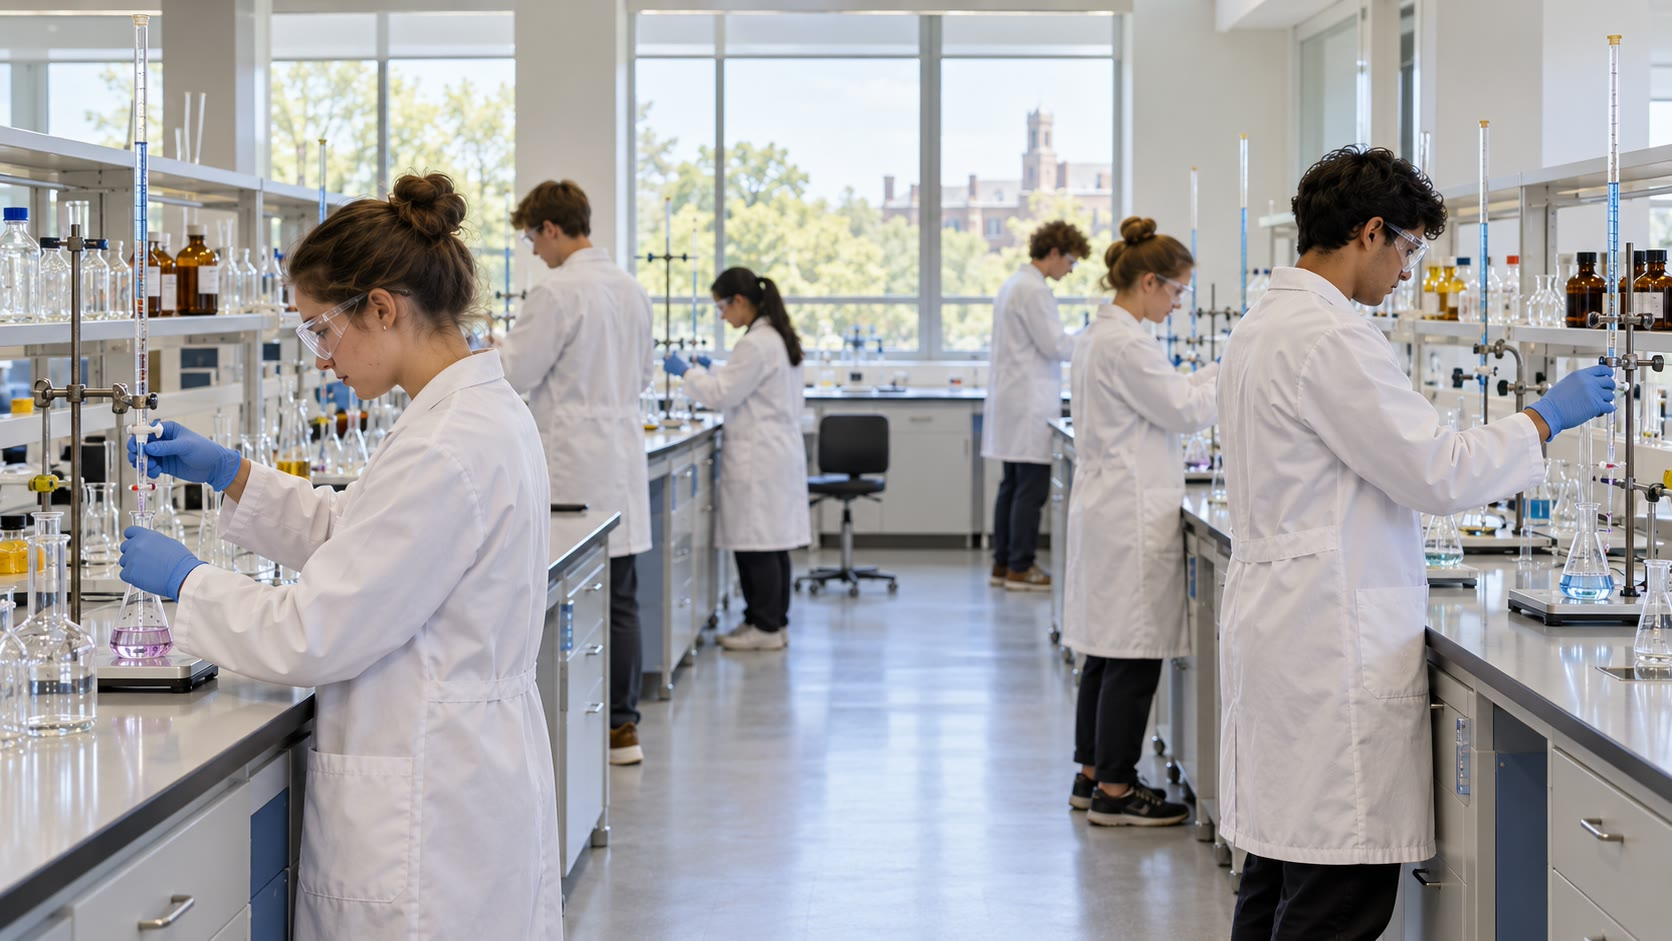
\includegraphics[width=0.66\linewidth]{images/book2/ai/b1-15-teaching-lab.jpg}

{\small Un laboratorio de prácticas: una bureta, un matraz Erlenmeyer
sobre un agitador magnético, guantes y gafas. Una \omterm{def:b1:titration-methods:titration}{valoración} es la medida
cuantitativa más corriente en química.}
\end{omfigure}

\section{Valoración y equivalencia}

\begin{definition}[Valoración, equivalencia]\label{def:b1:titration-methods:titration}
Una \emph{valoración}\index{valoracion@valoración} determina la cantidad de una
especie, el \emph{analito}\index{analito}, mediante una reacción con un
reactivo de concentración conocida, el \emph{valorante}\index{valorante},
que se añade progresivamente. La reacción debe ser única, \omterm{def:b1:extent-q-and-k:quantitative}{cuantitativa}
($K$ grande) y rápida. La \emph{equivalencia}\index{equivalencia} se
alcanza cuando el valorante y el analito se han puesto en contacto en las
proporciones estequiométricas de la reacción; el volumen añadido entonces
es el volumen de equivalencia, y el punto de la curva de valoración
correspondiente a ese volumen es el \emph{punto de
equivalencia}\index{punto de equivalencia}. El volumen al que se detiene
el experimentador, al ver un cambio de color o una ruptura en una curva,
es el \emph{punto final}\index{punto final}; un buen método hace que
coincida con la equivalencia.
\end{definition}

\begin{proposition}[Relación de equivalencia]\label{prop:b1:titration-methods:equivalence}
Para una reacción de \omterm{def:b1:titration-methods:titration}{valoración} $a\,\mathrm{A} + b\,\mathrm{B} \to \cdots$,
con el \omterm{def:b1:titration-methods:titration}{analito} A ($n_A$ mol) y el \omterm{def:b1:titration-methods:titration}{valorante} B a la concentración $C_B$, el
volumen de \omterm{def:b1:titration-methods:titration}{equivalencia} cumple
\[
  \frac{n_A}{a} = \frac{C_B V_{\mathrm{eq}}}{b} .
\]
\end{proposition}

\begin{proof}
Sea $x$ el avance tras añadir un volumen $V$ de \omterm{def:b1:titration-methods:titration}{valorante}. Antes de la
\omterm{def:b1:titration-methods:titration}{equivalencia}, B es limitante y, como la reacción es \omterm{def:b1:extent-q-and-k:quantitative}{cuantitativa},
$x = C_BV/b$; después, A es limitante y $x = n_A/a$. La \omterm{def:b1:titration-methods:titration}{equivalencia} es el
volumen en el que ambos se agotan a la vez, $n_A - ax = 0$ y
$C_BV - bx = 0$: al eliminar $x$ se obtiene la relación.
\end{proof}

\section{Valoraciones directas e indirectas}

\begin{definition}[Tipos de valoración]\label{def:b1:titration-methods:kinds}
En una \emph{valoración directa}\index{valoracion directa@valoración directa} el \omterm{def:b1:titration-methods:titration}{valorante} reacciona
con el propio \omterm{def:b1:titration-methods:titration}{analito}. En una \emph{valoración por
retroceso}\index{valoracion por retroceso@valoración por retroceso} se añade al \omterm{def:b1:titration-methods:titration}{analito} un exceso
conocido de un reactivo, y se valora el exceso que queda. Cuando una
disolución contiene varios \omterm{def:b1:titration-methods:titration}{analitos} que reaccionan sucesivamente con el
\omterm{def:b1:titration-methods:titration}{valorante}, se miden mediante \emph{valoraciones
sucesivas}\index{valoraciones sucesivas}, una \omterm{def:b1:titration-methods:titration}{equivalencia} tras otra;
cuando reaccionan a la vez y dan una sola \omterm{def:b1:titration-methods:titration}{equivalencia}, mediante una
\emph{valoración simultánea}\index{valoracion simultanea@valoración simultánea}, que solo da su suma.
\end{definition}

\begin{method}[Valoración por retroceso]\label{met:b1:titration-methods:back-titration}
Se usa cuando la reacción directa es lenta, cuando el \omterm{def:b1:titration-methods:titration}{analito} es
inestable o volátil, o cuando ningún indicador se adapta a la reacción
directa.
\begin{enumerate}
  \item Se añade una cantidad conocida $n_R$ de reactivo R, en exceso, y se
        deja que reaccione por completo con el \omterm{def:b1:titration-methods:titration}{analito} A
        ($\alpha\,\mathrm{A} + \rho\,\mathrm{R}$).
  \item Se valora el exceso de R con un \omterm{def:b1:titration-methods:titration}{valorante} T ($\rho'\,\mathrm{R} +
        \tau\,\mathrm{T}$) hasta el volumen de \omterm{def:b1:titration-methods:titration}{equivalencia} $V_T$.
  \item Se calcula $n_{R,\text{exceso}} = \frac{\rho'}{\tau}C_TV_T$ y, después,
        $n_A = \frac{\alpha}{\rho}(n_R - n_{R,\text{exceso}})$.
\end{enumerate}
\end{method}

El problema de fin de semana valora así la vitamina C: el ácido ascórbico
reduce un exceso de yodo, y el yodo que queda se valora con tiosulfato.

\section{Valoraciones pHmétricas e indicadores}

\begin{omfigure}
\begin{tikzpicture}[font=\small]
  \pic at (0,0) {stirrer};
  \pic at (0,0.18) {beaker={0.55}{omDef!14}};
  \pic at (0.2,2.45) {burette={0.75}{white}};
  \pic at (-0.45,0.45) {probe};
  \pic (m) at (-2.6,3.2) {meter={pH}};
  \draw[thick] (-0.45,3.45) to[out=90, in=0] (m-b);
  \node[anchor=west] at (0.65,6.2) {bureta: NaOH, \qty{0.100}{mol/L}};
  \node[anchor=west] at (1.0,1.0) {ácido, $V_0 = \qty{10.0}{mL}$, diluido};
  \draw[<-, omProp, thick] (1.2,-0.25) -- (1.8,-0.25) node[anchor=west, text=black] {agitador magnético};
  \draw[<-, omProp, thick] (-0.62,2.4) -- (-1.5,2.0) node[anchor=east, text=black] {electrodo combinado};
\end{tikzpicture}

{\small Una \omterm{def:b1:titration-methods:titration}{valoración} pHmétrica. El electrodo combinado de vidrio mide
el pH tras cada adición desde la bureta; el agitador mezcla la
disolución. El electrodo se calibra previamente con dos \omterm{def:b1:predominant-reaction:buffer}{disoluciones
tampón}.}
\end{omfigure}

\begin{omfigure}
\begin{tikzpicture}
\begin{axis}[name=s,
  width=0.5\linewidth, height=5.6cm, xmin=0, xmax=20, ymin=0, ymax=14,
  axis x line=bottom, axis y line=left, xlabel={$V$ (mL)}, ylabel={pH},
  xtick={0,5,10,15,20}, ytick={0,2,4,6,8,10,12,14},
  tick label style={font=\small}, label style={font=\small}]
\addplot[omDef, very thick] table[x=V, y=pH] {figdata/out/bachelor-1-titration-curves-strong.dat};
\addplot[omProp, thick] table[x=V, y=pH] {figdata/out/bachelor-1-titration-curves-weak.dat};
\node[font=\scriptsize, omDef, anchor=south west] at (axis cs:6,0.2) {\ce{HCl}};
\node[font=\scriptsize, omProp, anchor=west] at (axis cs:0.4,6.4) {\ce{CH3COOH}};
\draw[dotted] (axis cs:5,0) -- (axis cs:5,4.76) -- (axis cs:0,4.76);
\node[font=\scriptsize, anchor=north] at (axis cs:2.5,4.7) {$\mathrm{p}K_a$};
\end{axis}
\begin{axis}[at={(s.east)}, anchor=west, xshift=1.2cm,
  width=0.5\linewidth, height=5.6cm, xmin=0, xmax=20, ymin=0, ymax=14,
  axis x line=bottom, axis y line=left, xlabel={$V$ (mL)}, ylabel={pH},
  xtick={0,5,10,15,20}, ytick={0,2,4,6,8,10,12,14},
  tick label style={font=\small}, label style={font=\small}]
\addplot[omMeth, very thick] table[x=V, y=pH] {figdata/out/bachelor-1-titration-curves-mixture.dat};
\node[font=\scriptsize, anchor=west, align=left] at (axis cs:10.8,6.0) {\ce{HCl} + \ce{CH3COOH}\\ dos equivalencias};
\end{axis}
\end{tikzpicture}

{\small A la izquierda, \qty{10.0}{mL} de ácido clorhídrico y de ácido
etanoico, ambos de \qty{0.100}{mol/L}, valorados con hidróxido de sodio
de \qty{0.100}{mol/L}. El \omterm{def:b1:predominant-reaction:strong-acid}{ácido débil} presenta una zona tampón con pH $=
\mathrm{p}K_a$ en la semiequivalencia y un \omterm{def:b1:titration-methods:titration}{punto de equivalencia} a pH
8.73. A la derecha, una mezcla de \qty{0.050}{mol/L} de cada ácido: el
\omterm{def:b1:predominant-reaction:strong-acid}{ácido fuerte} se valora primero (\omterm{def:b1:titration-methods:titration}{equivalencia} a \qty{5}{mL}) y después el
débil (\qty{10}{mL}).}
\end{omfigure}

\begin{proposition}[Semiequivalencia de un ácido débil]\label{prop:b1:titration-methods:half-equivalence}
Cuando se valora un \omterm{def:b1:predominant-reaction:strong-acid}{ácido débil} HA con una \omterm{def:b1:predominant-reaction:strong-acid}{base fuerte}, en la
semiequivalencia $\mathrm{pH} = \mathrm{p}K_a$, siempre que el ácido no
sea ni demasiado fuerte ni demasiado diluido ($\mathrm{p}K_a$
aproximadamente entre 4 y 10 a \qty{0.1}{mol/L}).
\end{proposition}

\begin{proof}
En la semiequivalencia, la \omterm{def:b1:extent-q-and-k:quantitative}{reacción cuantitativa} \ce{HA + OH- -> A- + H2O}
ha convertido la mitad de HA: $[\mathrm{HA}] = [\mathrm{A^-}]$, y la
relación de Henderson da $\mathrm{pH} = \mathrm{p}K_a$. La condición
garantiza que la reacción de HA con el agua y la de $\mathrm{A^-}$ con el
agua no modifican apreciablemente esas cantidades.
\end{proof}

\begin{proposition}[pH en la equivalencia de un ácido débil]\label{prop:b1:titration-methods:ph-at-equivalence}
En la \omterm{def:b1:titration-methods:titration}{equivalencia} de un \omterm{def:b1:predominant-reaction:strong-acid}{ácido débil} ($\mathrm{p}K_a$) con una \omterm{def:b1:predominant-reaction:strong-acid}{base
fuerte}, la disolución es la base conjugada a la concentración $C'$ (tras
la dilución), y
\[
  \mathrm{pH} = \tfrac12(\mathrm{p}K_e + \mathrm{p}K_a + \log C') .
\]
\end{proposition}

\begin{proof}
La \omterm{def:b1:predominant-reaction:predominant-reaction}{reacción predominante} de la base con el agua,
\ce{A- + H2O <=> HA + OH-}, tiene $K = K_e/K_a$; con poca base
transformada, $[\ce{OH-}] = \sqrt{KC'}$ (\cref{prop:b1:predominant-reaction:ph-formulas}),
de donde el resultado. Para el ácido etanoico, $C' = \qty{0.050}{mol/L}$:
$\frac12(14.00 + 4.76 - 1.30) = 8.73$.
\end{proof}

\begin{proposition}[Valoraciones sucesivas]\label{prop:b1:titration-methods:successive}
Dos ácidos valorados con la misma base dan \omterm{def:b1:titration-methods:titration}{equivalencias} separadas, cada
una con un error inferior al \qty{1}{\percent}, si sus $\mathrm{p}K_a$
difieren en al menos 4.
\end{proposition}

\begin{proof}
En la primera \omterm{def:b1:titration-methods:titration}{equivalencia}, la reacción de la base $\mathrm{A_1^-}$ con
el segundo ácido $\mathrm{HA_2}$, $\mathrm{A_1^-} + \mathrm{HA_2}
\rightleftharpoons \mathrm{HA_1} + \mathrm{A_2^-}$, tiene $K = 10^{\mathrm{p}K_1 - \mathrm{p}K_2}$.
Partiendo de cantidades iguales, la fracción $x$ del segundo ácido ya
valorada cumple $x^2/(1 - x)^2 = K$; para $x \leqslant 0.01$, $K
\leqslant 10^{-4}$, es decir, $\mathrm{p}K_2 - \mathrm{p}K_1 \geqslant 4$.
\end{proof}

El ácido fosfórico (2.15, 7.21, 12.34) da dos \omterm{def:b1:titration-methods:titration}{equivalencias} claras; la
tercera se pierde en el agua de la base. El ácido etanoico mezclado con
ácido clorhídrico (a la derecha de la figura) se valora después de este,
pues el \omterm{def:b1:predominant-reaction:strong-acid}{ácido fuerte} equivale a un $\mathrm{p}K_a$ inferior a 0.

\begin{method}[Localizar una equivalencia en una curva]\label{met:b1:titration-methods:derivative}
\begin{enumerate}
  \item Derivada: se calcula $\Delta\mathrm{pH}/\Delta V$ entre puntos
        sucesivos; la \omterm{def:b1:titration-methods:titration}{equivalencia} está en su máximo.
  \item Tangentes: se trazan dos tangentes paralelas a la curva a cada
        lado del salto, y la paralela equidistante de ambas; esta corta
        la curva en el \omterm{def:b1:titration-methods:titration}{punto de equivalencia}.
\end{enumerate}
\end{method}

\begin{method}[Las tangentes, por cálculo]\label{met:b1:titration-methods:tangents}
Para una curva registrada por ordenador, se ajustan los puntos de cada
lado del salto con una función suave y se toma el punto de inflexión;
para un salto simétrico (\omterm{def:b1:predominant-reaction:strong-acid}{ácido fuerte}, \omterm{def:b1:predominant-reaction:strong-acid}{base fuerte}), el punto medio del
salto, a pH 7, es el \omterm{def:b1:titration-methods:titration}{punto de equivalencia}.
\end{method}

\begin{definition}[Indicador coloreado, zona de viraje]\label{def:b1:titration-methods:indicator}
Un \emph{indicador coloreado}\index{indicador coloreado} es un \omterm{def:b1:predominant-reaction:bronsted}{par
ácido--base} débil HIn/In$^-$ cuyas dos formas tienen colores distintos.
Su color cambia en la \emph{zona de viraje}\index{zona de viraje}, el
intervalo de pH en el que ninguna de las dos formas domina claramente,
aproximadamente $\mathrm{p}K_{a}(\mathrm{HIn}) \pm 1$.
\end{definition}

\begin{omfigure}
\begin{tabular}{lccl}
\hline
indicador & $\mathrm{p}K_a$ & \omterm{def:b1:titration-methods:indicator}{zona de viraje} & colores (ácido / base) \\
\hline
naranja de metilo & 3.5 & 2.5--4.5 & rojo / amarillo \\
rojo de metilo & 4.8 & 3.8--5.8 & rojo / amarillo \\
rojo de fenol & 7.9 & 6.9--8.9 & amarillo / rojo \\
azul de timol (segundo viraje) & 9.2 & 8.2--10.2 & amarillo / azul \\
\hline
\end{tabular}

\smallskip
{\small Cuatro indicadores, con $\mathrm{p}K_a$ tomados de una
recopilación crítica de \omterm{def:b1:complexation:formation-constant}{constantes de disociación}; las \omterm{def:b1:titration-methods:indicator}{zonas de viraje}
son $\mathrm{p}K_a \pm 1$.}
% ledger: pka:methylorange, pka:methylred, pka:phenolred, pka:thymolblue2
\end{omfigure}

\begin{method}[Elegir un indicador]\label{met:b1:titration-methods:choose-indicator}
Se elige un indicador cuya \omterm{def:b1:titration-methods:indicator}{zona de viraje} esté dentro del salto vertical
de la curva, lo más cerca posible del pH de la \omterm{def:b1:titration-methods:titration}{equivalencia}. \omterm{def:b1:predominant-reaction:strong-acid}{Ácido fuerte}
con \omterm{def:b1:predominant-reaction:strong-acid}{base fuerte} (salto de 3.3 a 10.7 para $\pm\qty{0.1}{mL}$ aquí):
cualquiera de los cuatro. Ácido etanoico (\omterm{def:b1:titration-methods:titration}{equivalencia} a 8.73): rojo de
fenol o azul de timol; el naranja de metilo cambiaría de color mucho antes
de la \omterm{def:b1:titration-methods:titration}{equivalencia}.
\end{method}

\section{Valoraciones potenciométricas}

\begin{definition}[Valoración potenciométrica]\label{def:b1:titration-methods:potentiometric}
Una \emph{valoración potenciométrica}\index{valoracion potenciometrica@valoración potenciométrica}
sigue el potencial de un electrodo sumergido en la disolución frente a un
\omterm{def:b1:nernst:reference-electrode}{electrodo de referencia}, en una \omterm{def:b1:titration-methods:titration}{valoración} redox (hilo de platino), de
precipitación (hilo de plata) o de complejación.
\end{definition}

\begin{proposition}[Puntos notables de una valoración redox]\label{prop:b1:titration-methods:potentiometric-points}
Para la \omterm{def:b1:titration-methods:titration}{valoración} de $\mathrm{Red_1}$ con $\mathrm{Ox_2}$ según
$n_2\,\mathrm{Red_1} + n_1\,\mathrm{Ox_2} \to n_2\,\mathrm{Ox_1} +
n_1\,\mathrm{Red_2}$ (pares de $n_1$ y $n_2$ electrones), $E(V_{\mathrm{eq}}/2) = E^\circ_1$, $E(2V_{\mathrm{eq}}) =
E^\circ_2$ y, en la \omterm{def:b1:titration-methods:titration}{equivalencia},
\[
  E_{\mathrm{eq}} = \frac{n_1E^\circ_1 + n_2E^\circ_2}{n_1 + n_2},
\]
para pares cuyas \omterm{def:b1:nernst:couple}{semiecuaciones} no contienen otras especies (o a un pH
que mantiene fijos los términos adicionales).
\end{proposition}

\begin{proof}
En la semiequivalencia, la mitad de $\mathrm{Red_1}$ está oxidada:
$[\mathrm{Ox_1}] = [\mathrm{Red_1}]$ y la \omterm{thm:b1:nernst:nernst}{ecuación de Nernst} del par 1 da
$E^\circ_1$. En $2V_{\mathrm{eq}}$ hay tanto $\mathrm{Ox_2}$ en exceso como
el que se redujo: $[\mathrm{Ox_2}] = [\mathrm{Red_2}]$, $E = E^\circ_2$.
En la \omterm{def:b1:titration-methods:titration}{equivalencia}, se multiplica la \omterm{thm:b1:nernst:nernst}{ecuación de Nernst} del par 1 por
$n_1$ y la del par 2 por $n_2$ y se suman; la estequiometría hace que
$[\mathrm{Ox_1}]/[\mathrm{Red_1}] \cdot [\mathrm{Ox_2}]/[\mathrm{Red_2}] = 1$
(las cantidades de $\mathrm{Red_1}$ y de $\mathrm{Ox_2}$ que quedan están
en la misma proporción que los productos), de modo que los logaritmos se
anulan.
\end{proof}

Para el hierro(II) con permanganato en ácido de \qty{1}{mol/L}, $n_1 = 1$
y $n_2 =
5$: $E_{\mathrm{eq}} = (0.77 + 5 \times 1.51)/6 = 1.39$~V. El salto, de
unos 0.8 a 1.5~V, es tan grande que el \omterm{def:b1:titration-methods:titration}{punto final} es nítido; en la
práctica, el permanganato es su propio indicador: su color violeta
persiste con la primera gota en exceso.

\begin{omfigure}
\begin{tikzpicture}
\begin{axis}[name=p,
  width=0.5\linewidth, height=5.6cm, xmin=0, xmax=20, ymin=0.6, ymax=1.6,
  axis x line=bottom, axis y line=left, xlabel={$V$ (mL)}, ylabel={$E$ (V)},
  xtick={0,5,10,15,20},
  tick label style={font=\small}, label style={font=\small}]
\addplot[omDef, very thick] table[x=V, y=E] {figdata/out/bachelor-1-titration-curves-potentiometric.dat};
\draw[dotted] (axis cs:5,0.6) -- (axis cs:5,0.77) -- (axis cs:0,0.77);
\draw[dotted] (axis cs:10,0.6) -- (axis cs:10,1.39) -- (axis cs:0,1.39);
\node[font=\scriptsize, anchor=south west] at (axis cs:0.2,0.77) {0.77};
\node[font=\scriptsize, anchor=south west] at (axis cs:0.2,1.39) {1.39};
\end{axis}
\begin{axis}[at={(p.east)}, anchor=west, xshift=1.2cm,
  width=0.5\linewidth, height=5.6cm, xmin=0, xmax=20, ymin=0, ymax=4.6,
  axis x line=bottom, axis y line=left, xlabel={$V$ (mL)},
  ylabel={$\kappa$ (mS/cm)}, xtick={0,5,10,15,20},
  tick label style={font=\small}, label style={font=\small}]
\addplot[omProp, very thick] table[x=V, y=kappa] {figdata/out/bachelor-1-titration-curves-conductimetric.dat};
\draw[dotted] (axis cs:10,0) -- (axis cs:10,1.15);
\end{axis}
\end{tikzpicture}

{\small A la izquierda, \omterm{def:b1:titration-methods:potentiometric}{valoración potenciométrica} de \qty{10.0}{mL} de
hierro(II) de \qty{0.100}{mol/L} con permanganato de \qty{0.0200}{mol/L}
en ácido de \qty{1}{mol/L} (electrodo de platino, potencial frente al
electrodo de hidrógeno). A la derecha, \omterm{def:b1:titration-methods:titration}{valoración} conductimétrica de
\qty{100}{mL} de ácido clorhídrico de \qty{0.0100}{mol/L} con hidróxido de
sodio de \qty{0.100}{mol/L}; la \omterm{def:b1:titration-methods:titration}{equivalencia} está en la intersección de
dos rectas.}
% ledger: lam:H+, lam:OH-, lamsalt:HCl, lamsalt:NaCl (conductivities in figdata/bachelor-1/titration-curves.py)
\end{omfigure}

\section{Valoraciones conductimétricas, complexométricas y de precipitación}

\begin{definition}[Conductividad molar iónica]\label{def:b1:titration-methods:conductivity}
La conductividad $\kappa$ de una disolución (en \unit{S/m}) mide lo bien
que transporta la corriente mediante el movimiento de sus iones. La
\emph{conductividad molar iónica}\index{conductividad molar ionica@conductividad molar iónica} $\lambda_i$ de
un ion es su contribución por mol y por unidad de volumen; su valor a
dilución infinita, $\lambda_i^\circ$, es una constante del ion y del
disolvente a una temperatura dada.
\end{definition}

\begin{proposition}[Ley de Kohlrausch]\label{prop:b1:titration-methods:kohlrausch}
En disolución diluida, la conductividad es la suma de las contribuciones
de los iones,
\[
  \kappa = \sum_i \lambda_i^\circ c_i ,
\]
la \emph{ley de Kohlrausch}\index{ley de Kohlrausch}; la conductividad
molar de una sal es la suma de las de sus iones.
\end{proposition}

\admitted{La \omterm{prop:b1:titration-methods:kohlrausch}{ley de Kohlrausch} expresa que los iones diluidos se mueven
de forma independiente; sus límites a concentraciones más altas se
estudian en el volumen del segundo año. Aquí se usa como ley
experimental.}

\begin{proposition}[Pendientes de una valoración conductimétrica]\label{prop:b1:titration-methods:conductimetric-slopes}
Cuando se valora un \omterm{def:b1:predominant-reaction:strong-acid}{ácido fuerte} H$^+$X$^-$ con una \omterm{def:b1:predominant-reaction:strong-acid}{base fuerte}
Na$^+$OH$^-$ en un volumen grande (despreciando la dilución), la
conductividad varía linealmente con el volumen añadido, con una
pendiente proporcional a
$\lambda^\circ(\ce{Na+}) - \lambda^\circ(\ce{H+}) < 0$ antes de la
\omterm{def:b1:titration-methods:titration}{equivalencia} y a $\lambda^\circ(\ce{Na+}) + \lambda^\circ(\ce{OH-}) > 0$
después.
\end{proposition}

\begin{proof}
Antes de la \omterm{def:b1:titration-methods:titration}{equivalencia}, cada mol de hidróxido añadido elimina un mol de
\ce{H+} (\ce{H+ + OH- -> H2O}) y aporta un mol de \ce{Na+}; después de la
\omterm{def:b1:titration-methods:titration}{equivalencia}, añade un \ce{Na+} y un \ce{OH-}. \ce{X-} no cambia. Según la
\omterm{prop:b1:titration-methods:kohlrausch}{ley de Kohlrausch}, la conductividad varía en esas combinaciones de
$\lambda^\circ$ multiplicadas por la cantidad añadida y divididas por el
volumen (fijo).
\end{proof}

A partir de las conductividades límite, $\lambda^\circ(\ce{H+}) =
\qty{349.8}{S.cm^2/mol}$ y $\lambda^\circ(\ce{OH-}) = 198.3$, y de las de
las sales \ce{HCl} (426) y \ce{NaCl} (126.5), la \omterm{prop:b1:titration-methods:kohlrausch}{ley de Kohlrausch} da
$\lambda^\circ(\ce{Cl-}) = 426 - 349.8 = 76.2$ y $\lambda^\circ(\ce{Na+}) =
126.5 - 76.2 = 50.3$~\unit{S.cm^2/mol}. Los iones hidrógeno e hidróxido
conducen mucho mejor que los demás: la curva es una V muy marcada.

Las \omterm{def:b1:titration-methods:titration}{valoraciones} complexométricas usan el EDTA: a pH 10 (tampón
amoniacal), el calcio y el magnesio reaccionan con él \omterm{def:b1:extent-q-and-k:quantitative}{cuantitativamente}
(constantes condicionales del \cref{ch:b1:complexation}), y un indicador
que es él mismo un complejante débil del metal cambia de color cuando el
EDTA le arrebata los últimos iones metálicos --- la \omterm{def:b1:titration-methods:titration}{valoración} de la
dureza del agua. Las \omterm{def:b1:titration-methods:titration}{valoraciones} de precipitación usan iones plata: el
cloruro se valora con nitrato de plata con cromato como indicador
(\cref{exo:b1:precipitation:8}), o se sigue con un electrodo de plata
(\cref{ch:b1:nernst}). La precisión de todos estos resultados, fijada por
el material de vidrio y por el \omterm{def:b1:titration-methods:titration}{punto final}, se trata en el
\cref{ch:b1:lab-techniques-1}.

\section{Ejercicios}

\begin{exercise}[$\star$]\label{exo:b1:titration-methods:1}
\qty{20.0}{mL} de una disolución de hidróxido de sodio necesitan
\qty{12.4}{mL} de ácido clorhídrico de \qty{0.100}{mol/L}. Escríbanse la
reacción y su constante, y calcúlese la concentración de la base.
\end{exercise}

\begin{exercise}[$\star$]\label{exo:b1:titration-methods:2}
¿Qué indicador de la tabla conviene para la \omterm{def:b1:titration-methods:titration}{valoración} de amoniaco
(\qty{0.10}{mol/L}, $\mathrm{p}K_a = 9.25$) con ácido clorhídrico de
\qty{0.10}{mol/L}? Calcúlese primero el pH en la \omterm{def:b1:titration-methods:titration}{equivalencia}.
\end{exercise}

\begin{exercise}[$\star$]\label{exo:b1:titration-methods:3}
Se valoran \qty{10.0}{mL} de hierro(II) con permanganato de
\qty{0.0200}{mol/L}; el color violeta persiste a partir de
\qty{12.6}{mL}. Escríbase la reacción y calcúlese la concentración de
hierro(II).
\end{exercise}

\begin{exercise}[$\star$]\label{exo:b1:titration-methods:4}
Una muestra de agua de \qty{50.0}{mL} se valora con EDTA de
\qty{0.0100}{mol/L} a pH 10; la \omterm{def:b1:titration-methods:titration}{equivalencia} está en \qty{14.2}{mL}. El
EDTA reacciona mol a mol con el calcio y el magnesio. Calcúlese la
concentración total de estos dos iones. ¿Se trata de una \omterm{def:b1:titration-methods:kinds}{valoración
simultánea} o de \omterm{def:b1:titration-methods:kinds}{valoraciones sucesivas}?
\end{exercise}

\begin{exercise}[$\star\star$]\label{exo:b1:titration-methods:5}
Para la \omterm{def:b1:titration-methods:titration}{valoración} de \qty{10.0}{mL} de ácido etanoico de
\qty{0.100}{mol/L} con hidróxido de sodio de \qty{0.100}{mol/L},
calcúlese el pH a 0, 5.0, 10.0 y \qty{15.0}{mL} con los métodos del
\cref{ch:b1:predominant-reaction}, y compárese con la curva de este
capítulo.
\end{exercise}

\begin{exercise}[$\star\star$]\label{exo:b1:titration-methods:6}
Demuéstrese que una \omterm{def:b1:titration-methods:titration}{valoración} pHmétrica del ácido fosfórico con
hidróxido de sodio da dos saltos, y calcúlese el pH en cada \omterm{def:b1:titration-methods:titration}{equivalencia}
para un ácido de \qty{0.100}{mol/L} (\qty{10.0}{mL}, base de
\qty{0.100}{mol/L}). ¿Por qué no hay tercer salto?
\end{exercise}

\begin{exercise}[$\star\star$]\label{exo:b1:titration-methods:7}
Una mezcla de ácido clorhídrico y ácido etanoico (\qty{10.0}{mL}) se
valora con hidróxido de sodio de \qty{0.100}{mol/L}: dos \omterm{def:b1:titration-methods:titration}{equivalencias}, a
\qty{6.2}{mL} y a \qty{14.6}{mL}. Calcúlense las dos concentraciones.
¿Cuál es el pH a medio camino entre las dos \omterm{def:b1:titration-methods:titration}{equivalencias}?
\end{exercise}

\begin{exercise}[$\star\star$]\label{exo:b1:titration-methods:8}
Calcúlese el potencial del electrodo de platino en la \omterm{def:b1:titration-methods:titration}{valoración} de
hierro(II) con permanganato (datos del capítulo) a 2.0, 9.0, 11.0 y
\qty{20.0}{mL}.
\end{exercise}

\begin{exercise}[$\star\star$]\label{exo:b1:titration-methods:9}
Con la \omterm{prop:b1:titration-methods:kohlrausch}{ley de Kohlrausch} y los valores del capítulo, calcúlese la
conductividad del ácido clorhídrico valorado a 0, 10.0 y \qty{20.0}{mL}
de base (\qty{100}{mL} de ácido de \qty{0.0100}{mol/L}, base de
\qty{0.100}{mol/L}, teniendo en cuenta la dilución), y las dos pendientes.
\end{exercise}

\begin{exercise}[$\star\star\star$]\label{exo:b1:titration-methods:10}
Demuéstrese que la curva pHmétrica de un \omterm{def:b1:predominant-reaction:strong-acid}{ácido fuerte} valorado con una
\omterm{def:b1:predominant-reaction:strong-acid}{base fuerte} es simétrica respecto del \omterm{def:b1:titration-methods:titration}{punto de equivalencia} cuando se
desprecia la dilución, y calcúlese la amplitud del salto entre
$V_{\mathrm{eq}} \pm 0.1$~mL para la \omterm{def:b1:titration-methods:titration}{valoración} del capítulo. ¿Cómo
cambia si todas las concentraciones se dividen por 100?
\end{exercise}

\begin{exercise}[$\star\star\star$]\label{exo:b1:titration-methods:11}
Dedúzcase la ecuación de la curva potenciométrica del hierro(II) con
permanganato antes y después de la \omterm{def:b1:titration-methods:titration}{equivalencia}, y compruébense los tres
puntos notables de la
\cref{prop:b1:titration-methods:potentiometric-points}. ¿Cómo cambiaría
el potencial de \omterm{def:b1:titration-methods:titration}{equivalencia} a pH 1?
\end{exercise}

\begin{exercise}[$\star\star\star$]\label{exo:b1:titration-methods:12}
El cloruro de amonio (\qty{0.100}{mol/L}, $\mathrm{p}K_a = 9.25$) no
puede valorarse con exactitud con hidróxido de sodio y un indicador.
Explíquese a partir de la curva y propóngase después una \omterm{def:b1:titration-methods:kinds}{valoración por
retroceso}: exceso de hidróxido de sodio, eliminación del amoniaco por
ebullición y \omterm{def:b1:titration-methods:titration}{valoración} del hidróxido restante con ácido clorhídrico.
Escríbase el cálculo.
\end{exercise}

\section{Problema: ¿cuánta vitamina C tiene el comprimido?}

\begin{problem}[{Problema de fin de semana --- la reacción del yodo con el
ácido ascórbico, una valoración por retroceso con tiosulfato, el cálculo
del resultado y su incertidumbre, para terminar con la masa de ácido
ascórbico por comprimido}]
\label{pb:b1:titration-methods:1}
Se tritura un comprimido y se disuelve en agua en un matraz aforado de
\qty{100.0}{mL}. Se toma con una pipeta una alícuota de \qty{10.00}{mL} y
se le añaden \qty{20.00}{mL} de disolución de yodo de \qty{0.0250}{mol/L}
(en exceso). El yodo que queda se valora con tiosulfato de sodio de
\qty{0.0500}{mol/L} con almidón como indicador: el color azul desaparece
a \qty{8.90}{mL}. El ácido ascórbico es \ce{C6H8O6}
($M = \qty{176.0}{g/mol}$); el yodo lo oxida a \ce{C6H6O6}.
$E^\circ(\ce{I2}/\ce{I-}) = 0.53$~V,
$E^\circ(\ce{S4O6^2-}/\ce{S2O3^2-}) = 0.02$~V.

\medskip
\noindent\textbf{Parte I --- Las reacciones.}
\begin{enumerate}
  \item Escríbase la \omterm{def:b1:nernst:couple}{semiecuación} del par \ce{C6H6O6}/\ce{C6H8O6}.
  \item Escríbase la reacción del yodo con el ácido ascórbico.
  \item Dese el \omterm{def:b1:nernst:oxidation-number}{número de oxidación} del yodo en \ce{I2} y en \ce{I-}.
  \item Escríbase la reacción del yodo con el tiosulfato y calcúlese su
        constante.
  \item El almidón da con el yodo un color azul intenso. ¿Por qué
        desaparece el color exactamente en la \omterm{def:b1:titration-methods:titration}{equivalencia} de la
        \omterm{def:b1:titration-methods:titration}{valoración} con tiosulfato?
  \item El oxígeno del aire oxida lentamente el ácido ascórbico. ¿Por qué
        aconseja esto añadir el yodo de una vez, en exceso?
\end{enumerate}

\medskip
\noindent\textbf{Parte II --- ¿Por qué una \omterm{def:b1:titration-methods:kinds}{valoración por retroceso}?}
\begin{enumerate}[resume]
  \item ¿Qué exigiría una \omterm{def:b1:titration-methods:kinds}{valoración directa} del ácido ascórbico con
        yodo?
  \item Descríbase la \omterm{def:b1:titration-methods:kinds}{valoración por retroceso} como las tres etapas del
        \cref{met:b1:titration-methods:back-titration}.
  \item ¿Por qué debe estar el yodo en exceso? Compruébese con el
        resultado.
  \item ¿Por qué se normaliza la disolución de tiosulfato poco antes de
        usarla?
  \item La alícuota es de \qty{10.00}{mL} de \qty{100.0}{mL}: ¿cuál es el
        factor de dilución?
  \item ¿Qué material de vidrio dispensa los \qty{20.00}{mL} de disolución
        de yodo?
\end{enumerate}

\medskip
\noindent\textbf{Parte III --- El cálculo.}
\begin{enumerate}[resume]
  \item Calcúlese la cantidad de yodo introducida.
  \item Calcúlese la cantidad de tiosulfato utilizada.
  \item Dedúzcase la cantidad de yodo en exceso.
  \item Dedúzcase la cantidad de yodo que ha reaccionado con el ácido
        ascórbico.
  \item Calcúlese la cantidad de ácido ascórbico en la alícuota.
  \item Calcúlense la cantidad y, después, la masa de ácido ascórbico en
        el comprimido.
  \item Compárese con la etiqueta (\qty{500}{mg}).
\end{enumerate}

\medskip
\noindent\textbf{Parte IV --- ¿Con qué seguridad?}
Las tolerancias son: matraz \qty{100.0 \pm 0.1}{mL}, pipetas
\qty{10.00 \pm 0.02}{mL} y \qty{20.00 \pm 0.03}{mL}, lectura de la bureta
$\pm\qty{0.05}{mL}$; las dos concentraciones se conocen al
\qty{0.2}{\percent}.
\begin{enumerate}[resume]
  \item Exprésese $n(\text{ácido ascórbico})$ en el comprimido en función
        de las magnitudes medidas.
  \item ¿Qué incertidumbres relativas intervienen en la cantidad de yodo
        introducida y en la cantidad en exceso?
  \item ¿Por qué una diferencia de dos cantidades amplifica la
        incertidumbre relativa?
  \item Combinando las contribuciones como en el
        \cref{ch:b1:lab-techniques-1} (suma cuadrática), estímese la
        incertidumbre relativa del resultado.
  \item Dese la masa de ácido ascórbico por comprimido con su
        incertidumbre, con dos cifras significativas.
\end{enumerate}
\end{problem}
